\section{configobj::Missing\-Interpolation\-Option Class Reference}
\label{classconfigobj_1_1MissingInterpolationOption}\index{configobj::MissingInterpolationOption@{configobj::MissingInterpolationOption}}
Inheritance diagram for configobj::Missing\-Interpolation\-Option::\begin{figure}[H]
\begin{center}
\leavevmode
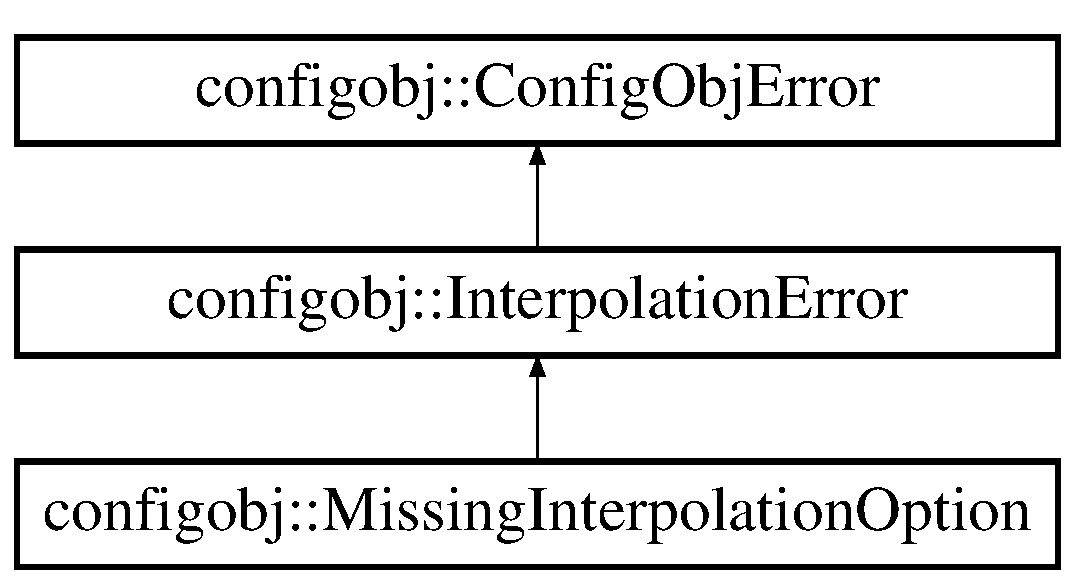
\includegraphics[height=3cm]{classconfigobj_1_1MissingInterpolationOption}
\end{center}
\end{figure}
\subsection*{Public Member Functions}
\begin{CompactItemize}
\item 
def \textbf{\_\-\_\-init\_\-\_\-}\label{classconfigobj_1_1MissingInterpolationOption_1cf2aab1dcc3b34cee7b65443c08d645}

\end{CompactItemize}


\subsection{Detailed Description}


\footnotesize\begin{verbatim}A value specified for interpolation was missing.\end{verbatim}
\normalsize
 



The documentation for this class was generated from the following file:\begin{CompactItemize}
\item 
old/PANICtool-1.0/configobj.py\end{CompactItemize}
